\documentclass[a4paper]{article}
\usepackage[T1]{fontenc}
\usepackage[utf8]{inputenc}
\usepackage[italian]{babel}
\usepackage{enumitem}
\usepackage{graphicx}
\graphicspath{{./images/}}
\usepackage{tabularx}
%\usepackage{geometry} 
%\geometry{a4paper,top=3cm,bottom=3cm,left=3.5cm,right=3.5cm,% heightrounded,bindingoffset=5mm}

\begin{document}

\author{Manuel Trivilino, Davide Salaorni, Luca Terracciano}

\title{\Large Data4Help\\
\Large RASD Requirements Analysis and Specification Document
}

\maketitle
\newpage

\tableofcontents
\newpage

\section{Introduction}

\subsection{Purpose}

\subsection{Scope}

\paragraph{Description of the given problem}

\paragraph{}
TrackMe is a company that develops software-based services for third parties and for consumers. The main service is called Data4Help.
 Data4Help is a service that allows third parties to monitor the location and the health status of individual, it handles a policy of permissions for each user and collects individual’s data from their personal devices.
The service supports the registration of individuals who, by registering, agree that TrackMe acquires their data. After registration, these third parties can request:

\begin{itemize}
    \item Access to the data of some specific individuals (we can assume, for instance, that they know an 
    individual by his/her social security number or fiscal code in Italy). In this case, TrackMe passes 
    the request to the specific individuals who can accept or refuse it.
    
    \item Access to anonymized data of groups of individuals (for instance, all those living in a certain 
    geographical area, all those of a specific age range, etc.). These requests are handled directly 
    by TrackMe that approves them if it is able to properly anonymize the requested data. For 
    instance, if the third party is asking for data about 10-year-old children living in a certain street 
    in Milano and the number of these children is two, then the third party could be able to derive 
    their identity simply having people monitoring the residents of the street between 8.00 and 
    9.00 when kids go to school. Then, to avoid this risk and the possibility of a misuse of data,
    TrackMe will not accept the request. For simplicity, we assume that TrackMe will accept any 
    request for which the number of individuals whose data satisfy the request is higher than 
    1000.

\end{itemize}

\paragraph{}
As soon as a request for data is approved, TrackMe makes the previously saved data available to the 
third party. Also, it allows the third party to subscribe to new data and to receive them as soon as 
they are produced.
TrackMe develops itself two third-party services: AutomatedSOS and Track4Run.

\paragraph{Goals}

\begin{enumerate}[label*={[G.\arabic*]}]
	
	%Data4Help
	
	\item Allow users to register in two different ways: single person and third parties.
	\item Third parties can request for users' data.
	    
	    \begin{enumerate}[label*=.\arabic*]
	        \item Third parties can request for anonymized data.
	        \item Third parties can request for a specific person's data.
	    \end{enumerate}
	    
	%AutomatedSOS
	\item Users' health status is continuously checked in AutomatedSOS and in case of it overcomes a certain threshold values an ambulance is called within 5 seconds.
	
	%Track4Run
	\item Users can organize a run.
	\item Users can enroll to a run.
	\item Users can be spectators of a run seeing the partecipants' position on a map.
	
\end{enumerate}

\subsection{Definitions, Acronyms, Abbreviation}


\subsection{Revision History}

\subsection{Reference Documents}

\subsection{Document Structure}

\section{Overall Description}

\subsection{Product Perspective}

\begin{figure}[h!]
    \centering
    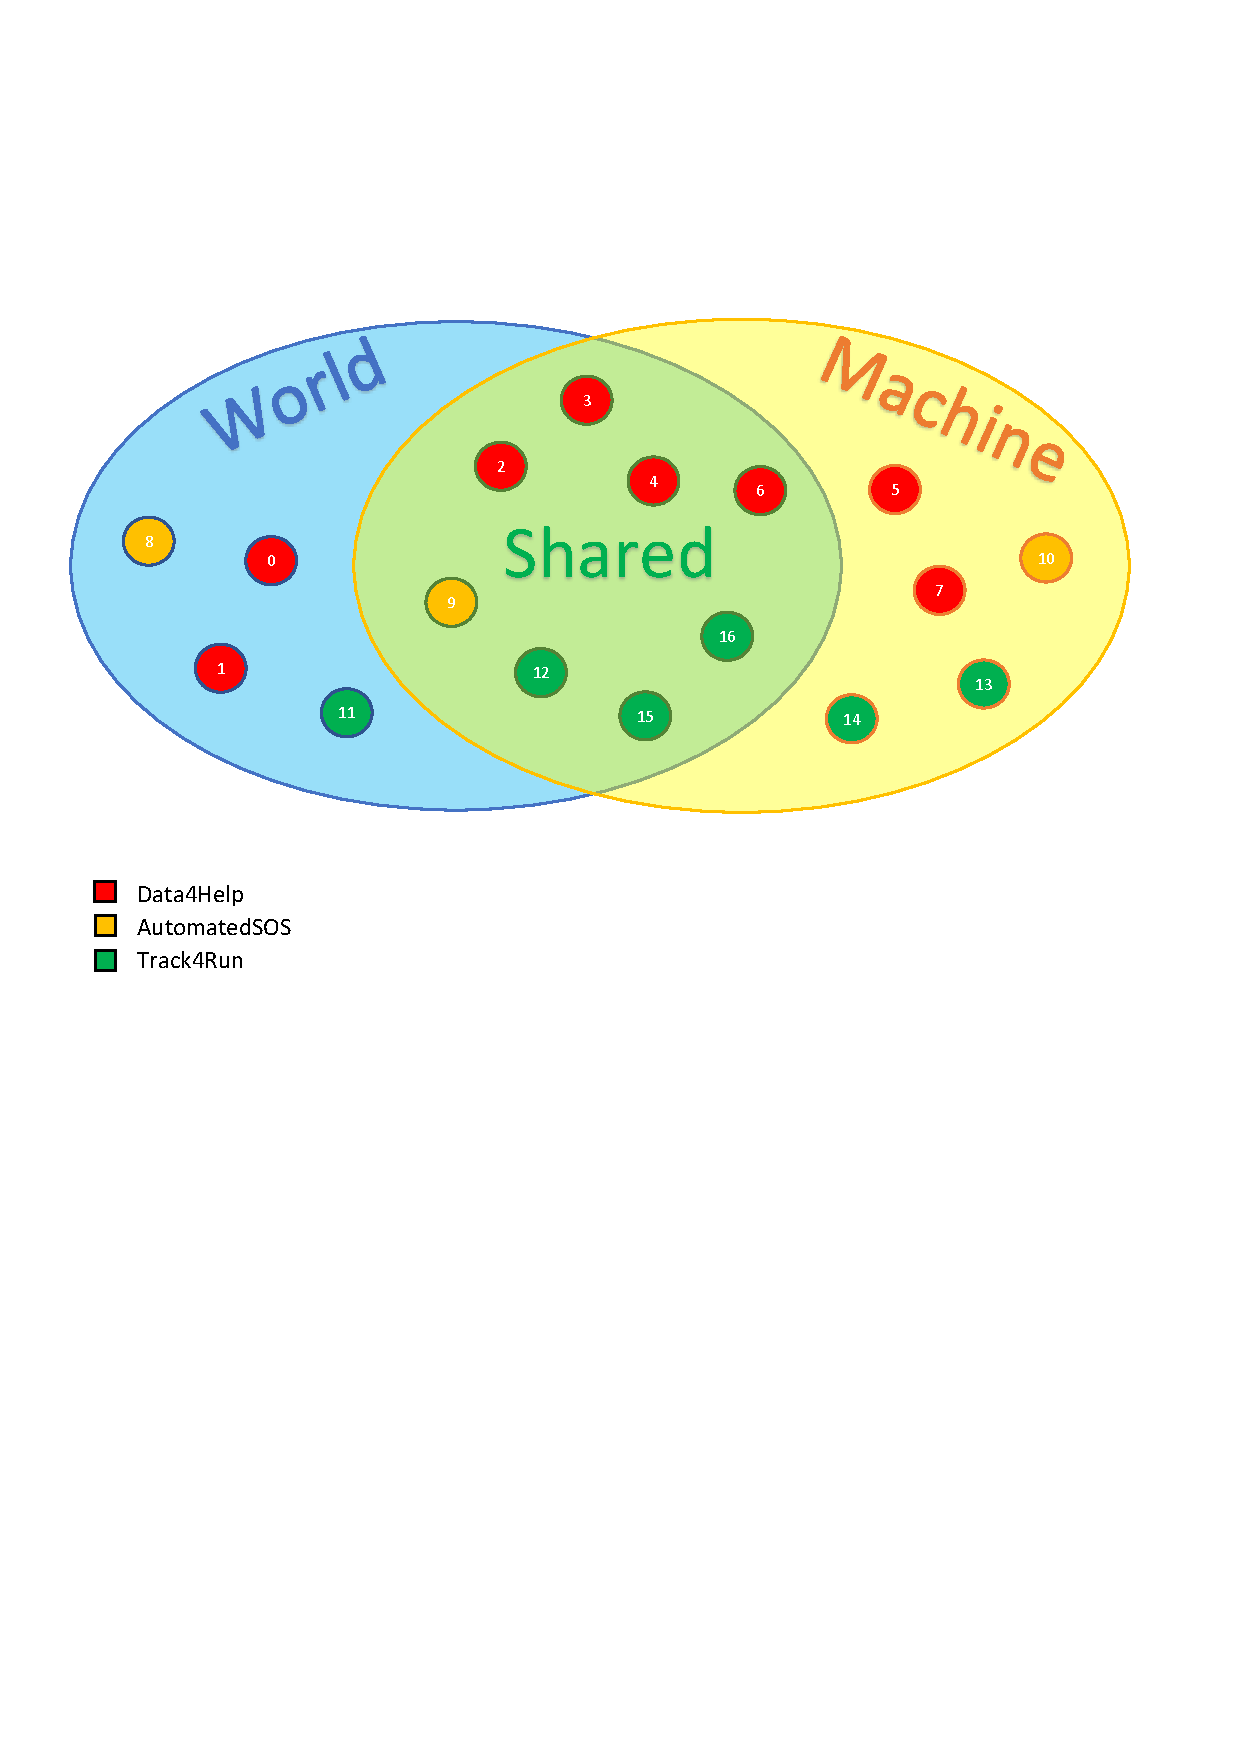
\includegraphics[width=\linewidth]{worldMachineShared-small}
    \caption{World, machine and shared phenomena.}
    \label{fig:my_label}
\end{figure}


\subsection{Product Functions}

\subsection{User Characteristics}

\paragraph{}The following actors are the users of the services offered by TrackMe. 


\begin{itemize}
    \item User:  a person that is successfully registered to TrackMe as consumer and allow to acquire anonymous data, eventually a client of third party services (i.e. AutomatedSOS, Track4Run) that allows even personal data.
    
    \item Third Parties:  a company or a person who is registred to TrackMe as "Third party" that access to anonymous and can require to access to individual data.
    
\end{itemize}

\subsection{Assumption, Dependencies and Constraints}

\subsubsection{Domain Assumptions}


\begin{enumerate}[label={[D.\arabic*]}]
    
    \item The data collected from the devices (position and health status) are reliable, accurate and in real time.
    \item Collected data belongs to the account owner and the personal informations (age, address, sex...) are correct.
    \item Ambulance call and information about patients' status and position are correctly dispatched to the ambulance contact center.
    
    
\end{enumerate}


\section{Specific Requirements}

\subsection{External Interface Requirements}

\subsubsection{User Interfaces}

\subsubsection{Hardware Interfaces}

\subsubsection{Software Interfaces}

\subsubsection{Communication Interfaces}

\subsection{Functional Requirements}

\begin{enumerate}[label*=\bf{G.\arabic*}]
	
	%Data4Help
	
	\item \textbf{Allow users to register in two different ways: single person and third parties.}
	
	\begin{enumerate}
	    \item [D.2] Collected data belongs to the account owner and the personal informations (age, address, sex...) are correct.
	    \item [R.1] People can create a user account selecting username, password, giving personal informations (age, address,sex) and allow to share their anonymized data.
	    \item [R.2] People or companies can a create third party account selecting username and password.
	\end{enumerate}
	
	\item Third parties can request for users' data.
	    
    \begin{enumerate}[label*=.\arabic*]
        \item Third parties can request for anonymized data.
	        
        \begin{enumerate}
	        \item [R.3] Data4Help allows requests for anonymized data from a group of users having certain characteristics (age, sex, address, etc.) from third parties.
            \item [R.4] Data4Help collects data from registered users and gives access to third parties only if the number of individuals whose data satisfy the request is higher than 1000.
            \item [D.2] Collected data belongs to the account owner and the personal informations (age, address, sex...) are correct.
            \item     
        \end{enumerate}

        \item Third parties can request for a specific person's data.
	        
        \begin{enumerate}
            \item [R.3] Users can accept or refuse third parties' request for individual data.
            \item [R.6] Data4Help keeps track of the connections between a specific user and the third parties that can access his/her data.
        \end{enumerate}
	        
    \end{enumerate}
	    
	%AutomatedSOS
	\item Users' health status is continuously checked in AutomatedSOS and in case of it overcomes a certain threshold values an ambulance is called within 5 seconds and sent to the user's position.

    \begin{enumerate}
        \item [D.1] The data collected from the devices (position and health status) are reliable, accurate and in real time.
        \item [R.7] Users' Health informations are collected from their devices and analyzed.
        \item [R.8] In case of emergency (the health status values overcome the threshold) a request fro an ambulance is sent to the ambulance contact center in 5 seconds, containing the information about user's health status and position.
        \item [D.3] Ambulance call and information about patients' status and position are correctly dispatched to the ambulance contact center.
    \end{enumerate}
	
	%Track4Run
	\item Users can organize a run.
	
	\begin{enumerate}
        \item [R.9] Users select the day, the hour at which the run begins, the starting point, the ending points and the path for the run.
        \item [R.10] The run event is stored in order to be managed when the run is about to start and during the run.
    \end{enumerate}
	
	\item Users can enroll to a run.
	
	\begin{enumerate}
        \item [R.11] Users can navigate among the the available runs and see their information.
        \item [R.12] Users can choice to see runs filtering them by city and/or date. 
        \item [R.13] The system saves the enrolled users as runners to the run event.
    \end{enumerate}
	
	\item Users can be spectators of a run seeing the participants' position on a map.
	
	\begin{enumerate}
        \item [R.14] The system keeps track of all the enrolled runners' position during the run.
        \item [R.15] Users who require to watch a run are saved as spectators to the run event.
    \end{enumerate}
	
\end{enumerate}

%Data4Help
\subsubsection{User's sign up}
\begin{center}
    \begin{tabular}{ l || p{6cm} ||}
        ACTORS & ciao \\ \hline
        GOALS & ciao \\ \hline
        ENTRY CONDITIONS & ciao come  \\ \hline
        EVENTS FLOW & ciao\\ \hline
        EXIT CONDITIONS & ciao\\ \hline
        EXCEPTIONS & ciao\\ \hline \hline
    \end{tabular}
\end{center}

\vspace{1cm}

\subsubsection{Request for anonymous data}
\begin{center}
    \begin{tabular}{l || p{6cm} ||}
        ACTORS & ciao faskjdkgajgdjgaskdgkagakjgkajgkaj fjdkjf gjsdaak djfsak fjakjfkda \\ \hline
        GOALS & ciao \\ \hline
        ENTRY CONDITIONS & ciao come  \\ \hline
        EVENTS FLOW & ciao\\ \hline
        EXIT CONDITIONS & ciao\\ \hline
        EXCEPTIONS & ciao\\ \hline \hline
    \end{tabular}
\end{center}

\vspace{1cm}

\subsubsection{Request for specific user's data}
\begin{center}
    \begin{tabular}{l || p{6cm} ||}
        ACTORS & ciao faskjdkgajgdjgaskdgkagakjgkajgkaj fjdkjf gjsdaak djfsak fjakjfkda \\ \hline
        GOALS & ciao \\ \hline
        ENTRY CONDITIONS & ciao come  \\ \hline
        EVENTS FLOW & ciao\\ \hline
        EXIT CONDITIONS & ciao\\ \hline
        EXCEPTIONS & ciao\\ \hline \hline
    \end{tabular}
\end{center}

\vspace{1cm}

%AutomatedSOS
\subsubsection{Alert emergency status}
\begin{center}
    \begin{tabular}{l || p{6cm} ||}
        ACTORS & ciao faskjdkgajgdjgaskdgkagakjgkajgkaj fjdkjf gjsdaak djfsak fjakjfkda \\ \hline
        GOALS & ciao \\ \hline
        ENTRY CONDITIONS & ciao come  \\ \hline
        EVENTS FLOW & ciao\\ \hline
        EXIT CONDITIONS & ciao\\ \hline
        EXCEPTIONS & ciao\\ \hline \hline
    \end{tabular}
\end{center}

\vspace{1cm}

%Track4Run
\subsubsection{Creation of a run event}
\begin{center}
    \begin{tabular}{l || p{6cm} ||}
        ACTORS & ciao faskjdkgajgdjgaskdgkagakjgkajgkaj fjdkjf gjsdaak djfsak fjakjfkda \\ \hline
        GOALS & ciao \\ \hline
        ENTRY CONDITIONS & ciao come  \\ \hline
        EVENTS FLOW & ciao\\ \hline
        EXIT CONDITIONS & ciao\\ \hline
        EXCEPTIONS & ciao\\ \hline \hline
    \end{tabular}
\end{center}

\vspace{1cm}

\subsubsection{Enrollment in a run}
\begin{center}
    \begin{tabular}{l || p{6cm} ||}
        ACTORS & ciao faskjdkgajgdjgaskdgkagakjgkajgkaj fjdkjf gjsdaak djfsak fjakjfkda \\ \hline
        GOALS & ciao \\ \hline
        ENTRY CONDITIONS & ciao come  \\ \hline
        EVENTS FLOW & ciao\\ \hline
        EXIT CONDITIONS & ciao\\ \hline
        EXCEPTIONS & ciao\\ \hline \hline
    \end{tabular}
\end{center}

\vspace{1cm}

\subsubsection{Specatation of a run}
\begin{center}
    \begin{tabular}{l || p{6cm} ||}
        ACTORS & ciao faskjdkgajgdjgaskdgkagakjgkajgkaj fjdkjf gjsdaak djfsak fjakjfkda \\ \hline
        GOALS & ciao \\ \hline
        ENTRY CONDITIONS & ciao come  \\ \hline
        EVENTS FLOW & ciao\\ \hline
        EXIT CONDITIONS & ciao\\ \hline
        EXCEPTIONS & ciao\\ \hline \hline
    \end{tabular}
\end{center}

\subsection{Performance Requirements}

\subsection{Design Constraints}

\subsubsection{Standards Compliance}

\subsubsection{Hardware Limitations}

\subsubsection{Any other Constraint}

\subsection{Software System Attributes}

\subsubsection{Reliability}

\subsubsection{Availability}

\subsubsection{Security}

\subsubsection{Maintainability}

\subsubsection{Portability}

\section{Formal Analysis Using Alloy}

\section{Effort Spent}

\section{References}


\end{document}